\documentclass[tikz,border=2pt]{standalone}
\usepackage{amsmath}
\usepackage{pgfplots}
\pgfplotsset{compat=1.18}

\begin{document}
% The indicator of A=[1,3]: value 1 on A, value 0 elsewhere, with jumps at the endpoints.
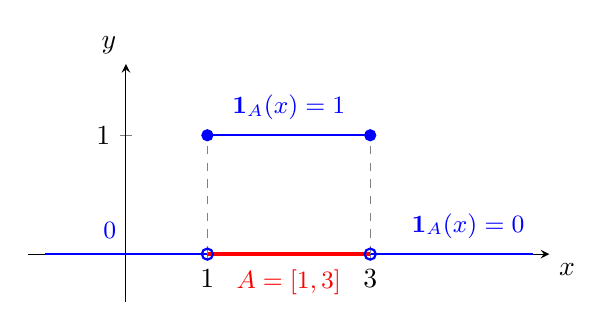
\begin{tikzpicture}
	\begin{axis}[
		axis lines=middle,
		xmin=-1.2, xmax=5.2,
		ymin=-0.4, ymax=1.6,
		xtick={1,3}, ytick={1},
		xlabel={$x$}, ylabel={$y$},
		xlabel style={below right}, ylabel style={above left},
		clip=false,
		width=8.2cm, height=4.6cm
		]
		\draw[very thick, red] (axis cs:1,0) -- (axis cs:3,0);
		\node[red, anchor=north, font=\small] at (axis cs:2,-0.05) {$A=[1,3]$};
		\addplot[thick, blue, samples=2, domain=-1:1] {0};
		\addplot[thick, blue, samples=2, domain=1:3] {1};
		\addplot[thick, blue, samples=2, domain=3:5] {0};
		\addplot[only marks, mark=*, blue] coordinates {(1,1) (3,1)};
		\addplot[only marks, mark=o, mark size=2pt, blue, thick, fill=white] coordinates {(1,0) (3,0)};
		\draw[dashed, gray] (axis cs:1,0) -- (axis cs:1,1);
		\draw[dashed, gray] (axis cs:3,0) -- (axis cs:3,1);
		\node[blue, anchor=south, font=\small] at (axis cs:2,1.05) {$\mathbf{1}_A(x)=1$};
		\node[blue, anchor=south, font=\small] at (axis cs:4.2,0.05) {$\mathbf{1}_A(x)=0$};
		\node[blue, anchor=south, font=\small] at (axis cs:-0.2,0.05) {$0$};
	\end{axis}
\end{tikzpicture}
\end{document}
